\documentclass[11pt]{article}

\usepackage[utf8]{inputenc} % character encoding - you don't need to understand this

% below are a bunch of useful packages, it doesn't cost anything to include them all so you might as well
\usepackage{amsmath}		% lets you input equations in math mode
\usepackage{graphicx}		% lets you include images
\usepackage{enumerate}		% lets you make lists
\usepackage{hyperref}		% lets you make links
\usepackage{subcaption}     % if you want to use subcaptions
\usepackage[all]{hypcap}	% makes links refer to figures and not captions
\usepackage{relsize}		% lets you use relative font sizes
\usepackage{caption}        % lets you add captions
\usepackage{array}          % lets you specify table column widths
\usepackage{siunitx}
\usepackage[margin=1in, paperwidth=8.5in, paperheight=11in]{geometry} % I'll bet you can figure this one out

% this line starts the actual document and text
\begin{document}

\title{ISIM Lab 2: An Analysis of Strain Sensors for Weight Measurement on the Surface of the Earth}
\author{Ari Porad}
% \date{date here} % leave this commented to display the current date
\maketitle % don't forget to include this line or you won't have a document header

\begin{abstract}
    A strain sensor attached to an aluminium bar was used to measure the weight of several washers. A cal
\end{abstract}

\section{Methodology}

Each day, millions of people drink at least one cup of coffee. Of those coffee drinkers, a substantial portion add some form of cream\footnote{Many different additives are commonly used in addition to or instead of cow-dairy cream. Popular alternatives include regular cow milk, almond milk, and soy milk.} to their coffee. However, cream must be refrigerated to prevent spoilage and food-borne illness, meaning that it is cold when added to the coffee and thereby acts to cool the coffee. If the coffee is to be drunk immediately, this is rarely a significant issue--immediately after brewing, the coffee is too hot to drink anyways, so cream serves to cool the coffee to a drinkable temperature. However, many coffee drinkers make coffee at home before commuting to work,\footnote{Notwithstanding the ongoing coronavirus pandemic, which has been hugely problematic for introductory undergraduate electrical engineering project pretexts.} and wish to drink their coffee upon arrival. This presents a conundrum for the coffee drinker, who must decide whether to add cream before departure or post-arrival. Which will ultimately result in a hotter cup of coffee at drinking time?

For this experiment, we set out to answer the above age-old question. We studied two different coffee creaming regimes, each simulating a 15 minute brew-to-drink time window:

\begin{enumerate}
    \item Adding cream to the coffee immediately after brewing, before the commute (n = 1).
	\item Adding cream to the coffee after arriving at work (t = 10 minutes post brew), 5 minutes before drinking the coffee (n = 1).
\end{enumerate}

For each trial, we poured the 100C coffee (represented by water: 150 mL for Regime #1 and 140 mL for Regime #2) into a paper cup and inserted a thermistor. For Regime #1, we immediately added 40 mL of 20C cream (also represented by water). For Regime #2, we added an identical 40 mL of 20C cream, but after 10 minutes. The temperature of all trials was measured for 15 minutes after pouring the coffee.

\subsection{Data Collection}

Figure ~\ref{fig:circuit} shows a diagram of the circuit used to measure the coffee's temperature. It consists of two identical voltage divider circuits, each dividing 5V of $V_{in}$ across a $\SI{1000}{\ohm}$ upper resistor and the lower thermistor. Leads for a channel of an O-Scope were connected across each thermistor, and the voltage measured can be calculated as follows:

\begin{equation}
    V_{out} = V_{in} \frac{R_{thermistor}}{R_{upper} + R_{thermistor}}
\end{equation}

The thermistor's resistance can be calculated from the following formula, where $T$ is the temperature of the coffee in Kelvin: 

\begin{equation}
    R_{thermistor} = \SI{1000}{\ohm} \times e^{-3528 \left(\frac{1}{298} - \frac{1}{T}\right)}
\end{equation}

% here, I used \ref{} to reference the figure below. Continue reading below to see how referencing works

% use \begin{figure} and \end{figure} to include a figure
\begin{figure} [!ht]
% the "!ht" will tell LaTeX to try and put the figure here, and at the top of the next page if it doesn't fit here. Getting figures to show up where you want can be a pain

	\centering  % this centers the image
	
	\includegraphics[width=0.3\textwidth]{circuit-diagram.png}
	% here I put the width as a fraction of the text width. You can also use a set number of inches, mm, pt, etc.
	% the text in the curly brackets is the name of the file. If it doesn't work, try adding the file extension, e.g. .jpg
	
	\captionsetup{margin={0.28\textwidth,0.28\textwidth}}
	% by adding margins to your caption, you can make the caption wrap with your figures rather than at the normal text width
	
	\caption{\smaller{A diagram of the double voltage divider circuit used to measure the temperature of the coffee. Each voltage divider is connected to 5V of $V_{in}$, with a $\SI{1k}{\ohm}$ upper resister and the thermistor as the lower resistor.}}
	% always caption your figures!
	
	\label{fig:circuit}
	% the label here allows me to reference this figure in text anywhere in this document. By matching the text inside the curly brackets of \label{} here and \ref{} in a paragraph, LaTeX automatically inserts the correct figure number and creates a link between the number and the referenced figure. As good practice, always use "fig:" at the beginning of figure labels
\end{figure}

\section{Results}

\subsection{Temperatures}

Regime #1, where cream was added to the coffee immediately after brewing, resulted in significantly warmer temperatures at t = 15 minutes (51C vs. 46C, see Figure~\ref{fig:temperature}). From this, it can be determined that immediately creaming coffee is the thermally ideal coffee creaming regime. Additionally, the immediate-cream regime is logistically far simpler, and eliminates the possibility that a coffee drinker forgets to add cream to their coffee. The author of this paper can see no reason why anyone would ever follow Regime #2.

\begin{figure} [!ht]
	\centering 
	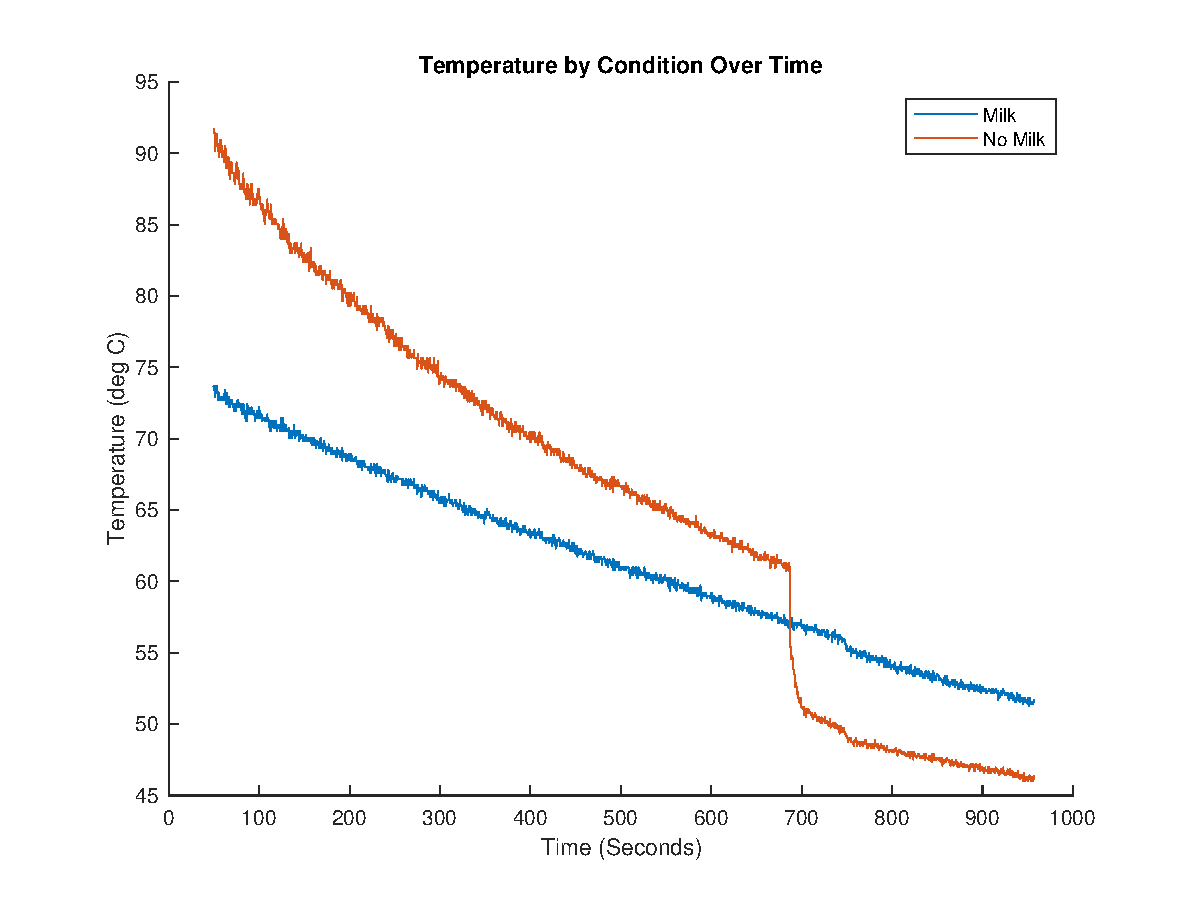
\includegraphics[width=0.7\textwidth]{isim1b.eps}
	\captionsetup{margin={0.2\textwidth,0.2\textwidth}}
	\caption{\smaller{Temperature over time by condition (creaming regime). Where cream was added immediately, the final temperature was much higher. Both regimes resulted in coffee that was barely above lukewarm.}}
	\label{fig:temperature}
\end{figure}

\begin{figure} [!ht]
	\centering 
	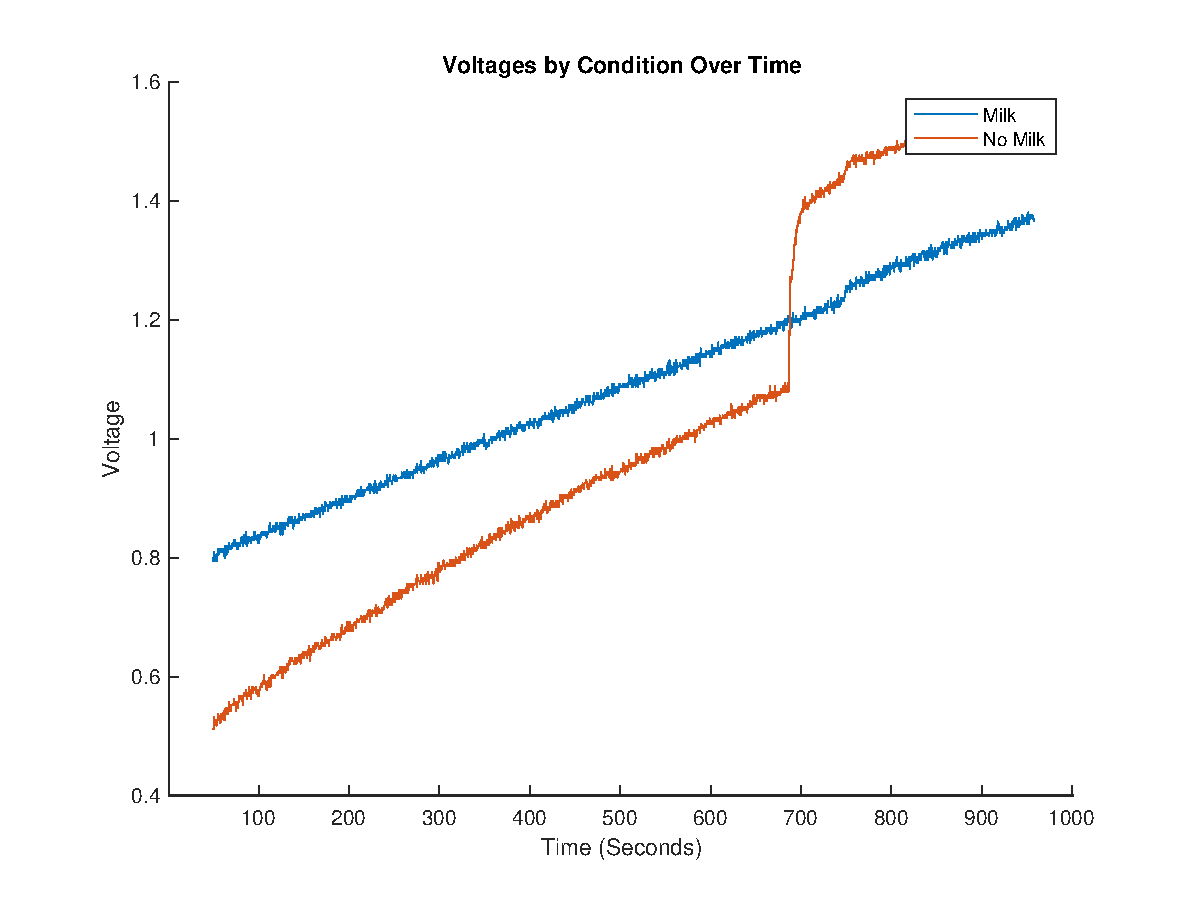
\includegraphics[width=0.7\textwidth]{isim1a.eps}
	\captionsetup{margin={0.2\textwidth,0.2\textwidth}}
	\caption{\smaller{Voltage over time by condition (creaming regime). Voltage is inversely proportional to temperature. Where cream was added immediately, the final voltage was much lower.}}
	\label{fig:voltage}
\end{figure}

\subsection{Model}

Additionally, we fitted a theoretical model of thermal convection cooling to our data (see Figure~\ref{fig:model}). The model is described by the following equation:

\begin{equation}
    22 + (T\left(0\right) - 22)e^{-t \over tau}
\end{equation}

We found the model to be relatively accurate. We only compared the model to Regime #1 (immediate milking), as the model would not have been able to predict the addition of cream at t = 10 minutes. During the experiment, the coffee was left undisturbed to eliminate any thermal effects from mixing. We calculated a parameter value of $\tau = 1752 \text{ seconds}$.

\begin{figure} [!ht]
	\centering 
	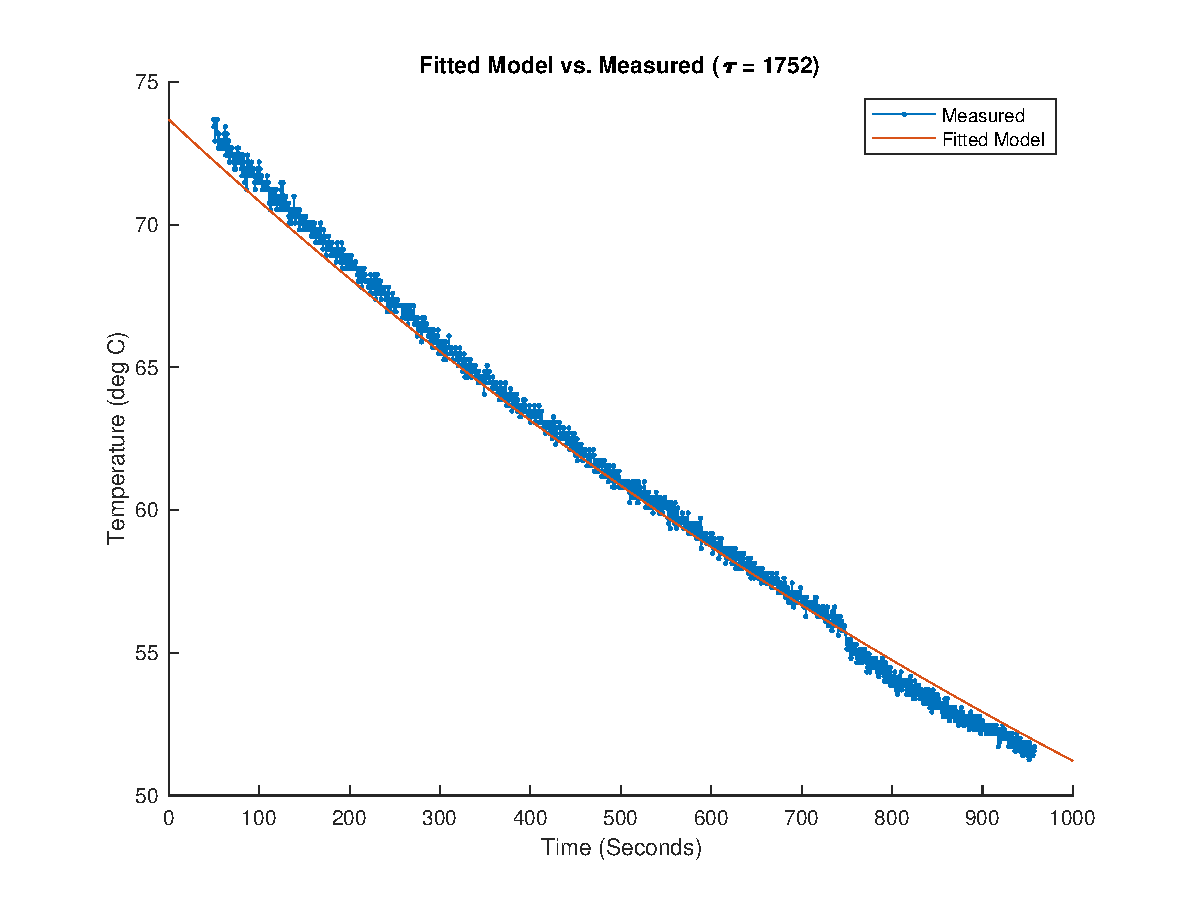
\includegraphics[width=0.7\textwidth]{isim1c.eps}
	\captionsetup{margin={0.2\textwidth,0.2\textwidth}}
	\caption{\smaller{Measured temperature (from the regime where the cream was added immediately vs a fitted theoretical model. The model does a reasonably good job of predicting the coffee's temperature. $\tau = 1752$}}
	\label{fig:model}
\end{figure}

\section{Finishing Remarks}
This experiment revealed several interesting conclusions about proper coffee creaming regimes. While the author has no doubt that this was a pedagogically useful lab, one cannot help but not that this absolutely constitutes "overthinking" one's morning coffee.\footnote{The other of this paper is from Seattle. Do you know what it takes to be ``overthinking coffee" in Seattle‽}
\end{document}